\section{Theory/Literature Review}\label{sec:Theory-Lit-Review}

Many of the individual things listed in this section are, in the land of computational physics, well known, meaning that many individual results aren't themselves are no longer worthy of being individually cited. Rather, a computational physics textbook like Ref.~\cite{Press_2007}.

\subsection{The Hard Scattering Process}

\subsubsection{Monte Carlo-Based Event Generators}

The driving force behind these types of simulation programs is the Monte Carlo algorithm, whose main purpose is to solve multi-dimensional integrals by averaging the integrand via randomly sampling points in the domain. Mathematically, what we are achieving is, given some integral

\begin{equation}
  I = \int_{t_1}^{t_2} \dd t \; f(t),
\end{equation}

we can approximate the result by

\begin{equation}
  I \approx \Delta t \Braket{f(t)} = \frac{\Delta t}{N} \sum_{\tau=1}^{\infty} f(\tau_i),
\end{equation}

where the $\tau_i$ lie in the range $(t_1,t_2)$. At this stage, we simply \textit{generate} $\tau_i$'s repeatedly, and the approximation will converge to the result. In practice, we can randomly generate a number in the range $(0,1)$, then scale it to the domain, something like

\begin{equation}
  \tau_i = (t_2 - t_1)\rho_i + t_1,
\end{equation}

where $\rho_i$ is the random number.

Of course, there are myriad other ways to solve integrals, but in particle physics, our problems and integrals are often formulated such that the dimensionality of the domain is large enough to dissuade the usage of quadrature-based integration schemes. Such integration schemes are more efficient in lower dimensions as they converge faster, but get much slower compared to Monte Carlo integration, whose rate of convergence increases in ``constant time'' in relation to the dimension. Of course, as an additional note, the reason this is a requirement at all is that the integrals we are faced with are very often mathematically impossible to solve analytically; e.g. the answer cannot be expressed in closed form.

Considering the physical process of the proton-proton collision, as mentioned before, the starting point is the hard scattering process, which occurs immediately after the collision. We make one assumption (admittedly a highly non-trivial one, but one that I have nowhere near enough time to explain) that at this energy scale, the physics related to the interaction amongst the quarks is independent of how the quarks are structured within the proton itself. In other words, we only care about the fact that the individual quarks carry only a fraction of the total momentum of the proton, and we can discard any other piece of information related to any other hadronic structure. With this assumption in mind, we can then write an expression for the \textit{cross section} $\sigma$ for proton-proton collisions. The cross section is, roughly speaking, the probability for a certain event to occur. It has units of area, so another way that this can be thought of is how much of a cross-sectional area the target provides to the other object (this is actually pretty much exactly what the cross section is). Intuitively, this still is roughly a probability: if the target is larger, i.e. the cross section is higher, there is a larger chance for the other particle to hit the target. The full expression is given as:\footnote{This formula, along with many of the following general results, can be found in any book on quantum field theory; see, for instance, Ref.\cite{peskin-schroeder}.}

\begin{equation}
  \sigma(p(P_1) + p(P_2) \rightarrow X + Y) = \int_0^1 \dd x_1 \int_0^1 \dd x_2 \; \sum_i f_{f_i}(x_1, \mu^2) f_{f_j}(x_2, \mu^2) \cdot \hat{\sigma}(f_j(x_1 P_1) + f_i(x_2 P_2) \rightarrow X).\label{eq:cross-section}
\end{equation}

Here, $P_1$ and $P_2$ are the incoming momenta of the protons $p$, $X$ is the immediate result of the scattering of the two partons $f_1$ and $f_2$, $Y$ is the generic hadronic state (which comes later), $x_1$ and $x_2$ are the momentum fractions that the parton carries with respect to its containing proton, and $\mu$ is an energy scale chosen to be characteristic of the reaction. The functions $f_{f_i}$ are the parton distribution functions mentioned earlier, and give probabilities that the parton $f_i$ will be found in the quark with momentum fraction $x_i$; $\hat{\sigma}$ is the \textit{partonic} cross section, which contains information related only to the interactions between the partons themselves. As I mentioned earlier, we have \textit{factorized} the information related to proton structure, that being the PDF factors, apart from the partonic structure, given by $\hat{\sigma}$.

The partonic cross section itself is given by the following integral:

\begin{equation}
  \dd\hat{\sigma}(f_i(x_1 P_1) + f_j(x_2 P_2) \rightarrow X) = \frac{1}{2\hat{s}} \abs{\mathcal{M}_{f_if_j \rightarrow X}}^2 \left( \prod_{k=1}^{N} \frac{\dd^3 p_k}{(2\pi)^3 2E_k} \right) (2\pi)^4 \delta^{(4)}(p_1 + p_2 + \sum_{k=1}^{N} p_k).
\end{equation}

Here, $N$ is the number of particles in the final state of the partonic subprocess, and $\hat{s} = x_1 x_2 s$ where $s$ is the center-of-mass energy for the partonic subprocess. $\mathcal{M}_{f_if_j \rightarrow X}$ is the \textit{matrix element} for the process, and is specific to the chosen process. This is also where considerations of how to incorporate corrections at higher orders will take place, as it is this matrix element that we must calculate perturbatively. Everything past this term in the above expression is called the \textit{phase space}, and for high $N$, we can see the high dimensionality of our domain.

Despite the main integral's intricacy, we can analytically calculate the individual components and then use Monte Carlo integration to get an approximate result. This is the main goal for the hard scattering process.

\subsubsection{The ``Hit-or-Miss'' Method}

In the event generation, when we are generating random phase space points and calculating our quantities of interest, we want to make sure that the events we are generating are in accordance with what would happen in the real world. In particular, if a phase space point gives a cross section significantly lower than others, it shouldn't necessarily be considered on the same footing as other events which are in principle far more likely to actually occur. One solution is to drag around every event's cross section so that we can take it into account later on. However, this extra baggage and additional computation can be inefficient.

One highly popular solution is dubbed the ``Hit-or-Miss'' method. This method involves finding the maximum ``weight'', which is the value of the integrand, during the calculation of the cross section; we shall call it $M_{\mathrm{max}}$. Then, when generating phase space points for the actual events, we only accept an event (it ``hits'') with a probability of $w/W_{\mathrm{max}}$, where $w$ is the weight of that event (otherwise it ``misses''). One caveat to this method is that it doesn't work well if the function is not flat. One way to imagine this is to consider a simple function/curve on the 2D plane and generate random $x$-values. Hits are those that land in/below the curve, and misses land outside/above it. Clearly, if the function isn't very flat, this method doesn't work well.

Sometimes, we are able to circumvent this by applying a transformation/change of variables. One particularly good example is the Breit-Wigner peak, modeled by the function

\begin{equation}
  F(m^2) = \frac{1}{(m^2 - M^2)^2 + M^2\Gamma^2}.
\end{equation}

This function is used to model resonances, which are essentially unstable particles, where $m^2$ is the center of mass energy that produces the resonance, $M$ is the actual mass of the resonance, and $\Gamma$ is the decay width of the resonance, which is inversely proportional to the lifetime of the particle. We are often interested in integrals of this function:

\begin{equation}
  I = \int_{M_{\mathrm{min}}^2}^{M_{\mathrm{max}}^2} \dd m^2 \; \frac{1}{(m^2 - M^2)^2 + M^2\Gamma^2}.
\end{equation}


\begin{figure}[ht]
  \centering
  
  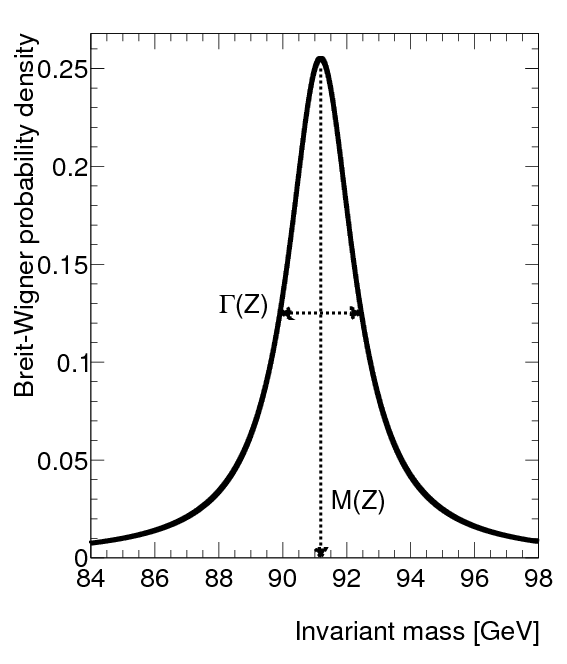
\includegraphics[width=0.4\linewidth]{./res/Images/breit-wigner.png}

  \caption{Example of the Breit-Wigner distribution.}
  \label{fig:BreitWigner}
\end{figure}


An example plot is given in Fig.~\ref{fig:BreitWigner}. Obviously, such a function would be a particularly bad candidate for the hit-or-miss method. However, if we made the change of variables to $\rho$ like so:

\begin{equation}
  m^2 = M\Gamma\tan\rho + M^2,
\end{equation}

our integral turns into

\begin{equation}
  I = \frac{1}{M\Gamma} \int_{\rho_{\mathrm{min}}}^{\rho_{\mathrm{max}}} \dd\rho,
\end{equation}

which is perfectly flat, thus removing any variance and making it a perfect candidate for the hit-or-miss method. Unfortunately, we are probably never going to be able to find a transformation that is perfect like this one, but we can often get very close, which is more than good enough, especially considering that we are already truncating things at leading-order anyways.

At this point, once we have a set of phase space points that passed the hit-or-miss selection, we can generate events by simply generating some momenta in accordance with the phase space information. These will correspond to particles that, in a real simulation, would be produced immediately after the collision. After this, we proceed to the parton showering part of the simulation.


\subsection{Parton Showering/Hadronization Process}

The calculation of hard scattering matrix elements and generation of events in accordance with the matrix elements is far more simple than the parton showering process, since the former is really an exercise in evaluating integrals with Monte Carlo algorithms. Parton showering is a little more based directly within the physics itself. As such, the results presented in this section are a conglomeration of results taken from the \textsc{Pythia8} and \textsc{Herwig7} manuals \cite{PYTHIA8DOC,HERWIGDOCS}, as well as from a condensed ``tutorial'' given in \cite{PYRESIAS}.

Once we have some reasonable particles from the hard scattering process, the next thing to consider is the possibility for these particles to radiate gluons/photons, called ``parton showering.'' In the leading-order limit, which I am considering at first, this is all that is involved; I will not be considering subsequent decays/annihilations.

The main mathematical structure related to the emission of gluons/photons is the \textit{Sudakov form factor}, defined like so:

\begin{equation}
  \Delta(t_0,t) \equiv \exp\left[ -\int_{t_0}^t \dd t' \; \Gamma(t') \right],
\end{equation}

where

\begin{equation}
  \Gamma(t') \equiv \frac{1}{t'} \int_{z_-}^{z_+} \dd z \; \frac{\alpha_s}{2\pi}P_{g \leftarrow q}(z).
\end{equation}

Here, $t'$ or $t$ is a generic evolution variable, usually an energy scale, and $t_0$ is a cutoff scale, since if we get to too low of an energy, i.e. the gluon we emit is too closely collinear or soft, meaning low energy, our integrals begin to diverge. $z$ is a momentum fraction, like $x_1$ or $x_2$ defined above, and the limits $z_+$ and $z_-$ are usually determined from the specific kinematics of the process under consideration. $\alpha_s$ is the strong coupling constant, and $P_{g \leftarrow q}(z)$ is called a \textit{splitting function} (specifically for a gluon splitting from a quark), defined like so:

\begin{equation}
  C_F \frac{1 + z^2}{1 - z},
\end{equation}

where $C_F=4/3$. The Sudakov form factor corresponds to the probability that the parton (quark in this case) \textit{doesn't} emit a gluon as we evolve from the initial scale $t$ to the cutoff scale $t_0$. This may seem backward, so to be sure: we are starting from the higher energy of the hard process $t$, and lowering the energy to the cutoff scale $t_0$.

So, one way that we can do the showering is by generating a random number in the range $[0,1]$, and comparing it to value of the Sudakov form factor for the range $(t_0,t_{\mathrm{max}}$, where $t_{\mathrm{max}}$ starts at the initial scale of the hard process). If we find an emission, the scale that it occurs becomes the new $t_{\mathrm{max}}$. In case our random number is greater, then that means we will have an emission, so we numerically solve the equation

\begin{equation}
  R = \Delta(t,t_{max})
\end{equation}

for $t$, which determines the evolution scale that the emission occurs at. Then, as I just mentioned, this becomes the new $t_{\mathrm{max}}$ and we continue the evolution until we reach our cutoff scale. Further, we need to determine/consider the kinematics of the emitted gluon, specifically $z$, the fraction of the parton's momentum it carries. This is done by solving for $z$ from $\Gamma(t)$ defined above.

There are a few issues with solving for $t$ and $z$, and that is the fact that both require evaluating inverses or integrals of functions which are, in general, very hard to integrate or invert. There is an algorithm to largely resolve this, called the \textit{Sudakov veto algorithm}. The main idea is that for the functions that we have to invert, we take away some of the complexity by defining new variables that are \textit{overestimates} of the original variable for the entire domain such that the function is more easily invertable. Of course, this implies a higher ``acceptance'' of events or of emissions. The probabilities are ``fixed'' by only accepting proposed events according a ratio of the original variable's value to the overestimate's value.

As an example, an overestimate of the splitting function would be given by

\begin{equation}
  \hat{P}(z) = C_F \frac{2}{1-z},
\end{equation}

and this function is more easily invertable.

In terms of actual functioning parts from within the algorithm that would be directly implemented in the code, we would be considering solving for $t$ (assuming a random $R$ greater than the value of the Sudakov form factor) from $R = \Delta(t,t_{\mathrm{max}})$. After doing some rearranging, we find the function

\begin{equation}
  E(t) = \log \frac{t}{t_{\mathrm{max}}} - \frac{1}{\rho} \log R,\label{eq:parton-shower-t}
\end{equation}

where

\begin{equation}
  \rho = t\hat{\Gamma}(t),
\end{equation}

where the hat indicates the overestimated quantity. The values of $t$ that we are interested in involve $E(t) = 0$, so we can employ traditional root-finding algorithms. One thing we can do to make it more efficient is use the entire logarithm term as the independent variable, then exponentiate and multiply by $t_{\mathrm{max}}$ to obtain $t$, rather than trying to make the root-finding algorithm do it. To find $z$, we can do some more rearranging to find

\begin{equation}
  z = \tilde{\rho}^{-1}\left( \tilde{\rho}(\hat{z}_- + R'[\tilde{\rho}(\hat{z}_+) - \tilde{\rho}(\hat{z}_-)] \right),\label{eq:parton-shower-z}
\end{equation}

where

\begin{equation}
  \tilde{\rho}(z) = \int^{z} \dd z \; \frac{\hat{\alpha}_s}{2\pi}\hat{P}(z),
\end{equation}

and again, the hats indicate the overesimated quantities.

To recap: we generate random numbers and compare to the Sudakov form factor to determine whether an emission occurs or not. If one does occur, we numerically solve for the value of $t$ using Eq.~\eqref{eq:parton-shower-t}. We generate the gluon and give it a momentum fraction $z$ via Eq.~\eqref{eq:parton-shower-z}. We then accept this new event based upon the ratio of the original to the overestimated quantities. Then, the scale $t$ that the emission occurred at becomes the new $t_{\mathrm{max}}$, and we continue until we reach our cutoff.

We are then left with some number of emitted gluons along with corresponding momenta and other kinematics. In higher-order limits, these would potentially scatter with other gluons or quarks, or possibly decay into quark/anti-quark pairs, and so on. After this, they would hadronize.



%%% Local Variables:
%%% mode: LaTeX
%%% TeX-master: "../../Report"
%%% End:
